\documentclass[12pt]{article}

\usepackage[T1]{fontenc}
\usepackage[utf8]{inputenc}
\usepackage[russian]{babel}

% page margin
\usepackage[top=2cm, bottom=2cm, left=2cm, right=2cm]{geometry}

% AMS packages
\usepackage{amsmath}
\usepackage{amssymb}
\usepackage{amsfonts}
\usepackage{amsthm}

\usepackage{float}
\usepackage{graphicx}
\usepackage{tabularx}

\newcommand{\lb}{\left(}
\newcommand{\rb}{\right)}

\makeatletter
\setlength{\@fptop}{0pt}
\makeatother

\begin{document} 

\begin{titlepage}
\centering
\textbf{\large Московский государственный университет имени М.В.\,Ломоносова\\
\vspace*{0.1cm} Химический факультет\\
\vspace*{0.1cm}
\noindent\makebox[\linewidth]{\rule{\paperwidth}{0.4pt}}
\vspace*{0.1cm}
 Кафедра физической химии}
\vspace*{2cm}

\begin{center}
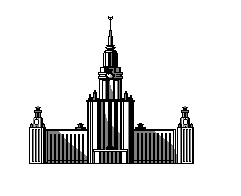
\includegraphics[width=0.3\textwidth]{pictures/logo.jpg}
\end{center}

\vspace*{2cm}
\Large \textbf{Сканирующая электронная микроскопия непроводящих материалов}
\vspace*{6cm}

\begin{flushright}
\large Работа выполнена студентом 515 группы\\
Финенко А.А.\\
\end{flushright}
\vfill
\large\textbf{Москва\\ 2017}
\end{titlepage}

\newpage
\section*{Теоретический вопрос}
4. Подготовка непроводящего  образца для СЭМ. Устройства для напыления металлического слоя. \par

Доля энергии падающего пучка электронов, которая выделяется в виде рентгеновского излучения, света и пр. очень невелика, большая же часть ее преобразуется в тепло и нагревает мишень. Хотя рассеянная (общая) мощность пучка составляет порядка милливатт, удельная мощность (приходящая на единицу площади) очень высокая, благодаря небольшому размеру бомбардируемой зоны. Температурный градиент $\Delta T$ можно оценить с помощью следующего выражения:

\begin{gather}
		\Delta T = 4.8 E_0 \cdot i / \lb k \cdot d \rb, 
\end{gather}
где $E_0$ -- энергия падающего электрона (кэВ); $i$ -- ток зонда (мкА); $k$ -- теплопроводность образца(Вт$\cdot$см$^{-1}\cdot$K$^{-1}$); $d$ -- диаметр пучка (мкм). 

\begin{figure}[!ht]
\centering
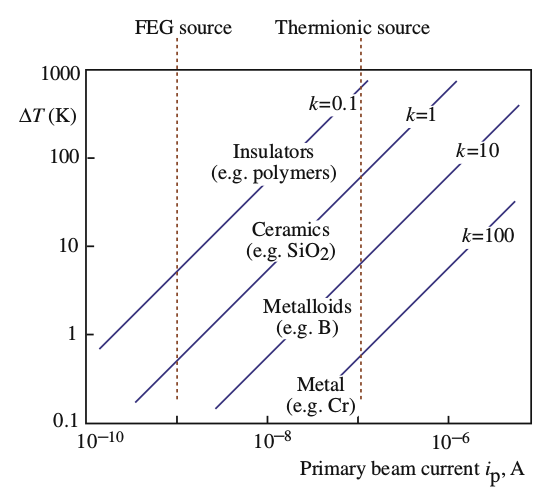
\includegraphics[scale = 0.7]{pictures/delta_t.png}
\caption{Рост температуры образца $\Delta T$ как функция тока зонда $I$ и теплопроводности образца $k$ в Вт $\cdot$ м$^{-1}$ $\cdot$ мK$^{-1}$.}
\label{tungsten-cathode}
\end{figure}

Для металлов величина $k$ обычно лежит в пределах от 1 до 4 Вт$\cdot$см$^{-1}\cdot$K$^{-1}$, и при нормальных условиях $\Delta T$ (пренебрежимо) мало. С другой стороны, для материалов с низкой теплопроводностью, включая многие минералы, температура может значительно возрастать, например, в случае слюды ($k = 6 \cdot 10^{-3}$ Вт$\cdot$см$^{-1}\cdot$K$^{-1}$) рассчитанный рост температурного градиента составляет $\Delta T = 160^\circ$C при $E_0 = 20$ кэВ, $i = 10$ нА и $d = 1$ мкм. Влияние нагрева может быть ослаблено следующими способами:
\begin{itemize}
		\item снижение тока 
		\item увеличение диаметра зонда 
		\item пократие образца слоем с высокой теплопроводностью
\end{itemize}

Нагрев образца можно снизить, применяя для напыления материал с высокой теплопроводностью (алюминимй, медь, золото, серебро, платина). При изучении рентгеновского спектра наиболее подходящим элементом для напыления является углерод, так как он имеет минимальный рентгеновский спектр. Однако при исследовании образца с помощью РЭМ он не распространен, т.к. углерод дает низкий выход вторичных электронов. В РЭМ предпочтительнее использовать металлы с высоким выходом вторичных электронов; наиболее распространены золото и золото-палладиевый сплав.  

\subsection*{Напыление углеродного покрытия}

При обычном способе напыления углеродного слоя образец помещается в вакуумной камеру с устройством для углеродного напыления, состоящим из двух графитовых стержней (диаметром 3-6 мм), которые постоянно легко прижаты друг к другу при помощи специальной пружины. Через стержни в течение несокльких секунд пропускается ток величиной порядка 100 А, вызывая испарение углерода из точки контакта стержней. Давление в вакуумной камере при этом должно быть меньше $10^{-2}$ Па, которое обычно достигается с помощью диффузионного насоса (редко, с помощью турбомолекулярного). При недостаточно низком вакууме углеродный слой получается "сажеобразный" и проявляет плохую адгезию к поверхности образца. Поскольку в процессе напыления атомы углерода перемещаются по прямой, такой способ напыления годится только для плоских образцов, но непригоден для образцов неправильной формы. В последнем случае качественное покрытие получается при вращении образца в процессе напыления. 

\begin{figure}[!ht]
\centering
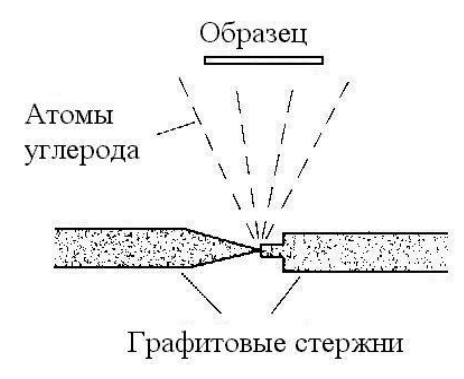
\includegraphics[scale = 0.5]{pictures/graphite.png}
\caption{Схема нанесения углеродного напыления на образец}
\label{tungsten-cathode}
\end{figure}

Оптимальная толщина углеродного слоя составляет около 20 нм. Примерный контроль толщины слоя осуществляют, используя фиксированный ток и вермя испарения. 

\subsection*{Напыление металлического слоя}

Наиболее распространенным металлом для напыления является золото, однако иногда рентгеновские линии золота попадают в изучаемый энергетический диапазон. Поэтому как альтернативу используют алюминий, медь или серебро. Эти металлы также можно напылять испарением в вакууме, используя вольфрамовую корзинку или молибденовую лодочку, которые нагреваются пропусканием тока. 

\begin{figure}[!ht]
\centering
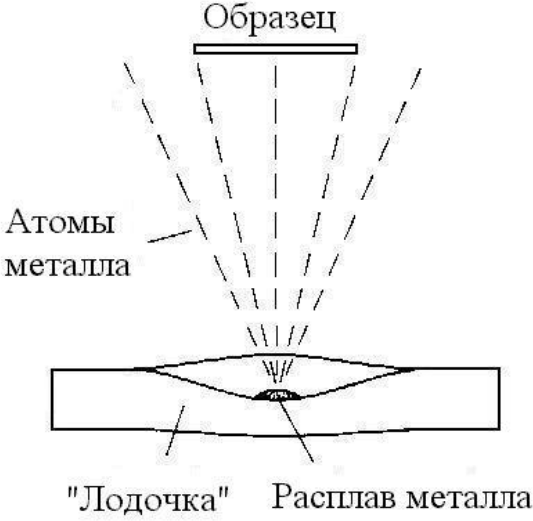
\includegraphics[scale = 0.5]{pictures/boat.png}
\caption{Напыление металла (серебра, алюминия) с помощью термического испарения в вакууме из молибденовой "лодочки"}
\end{figure}

Для получения проводящих слоев из золота или золото-палладиевого сплава применяют ионное напыление в вакууме. \par
С помощью форвакуумного насоса из камеры откачивается воздух и замещается аргоном до давления 10 Па. Когда на мишень подается высокое напряжение в камере начинается газо-разрядный процесс и мишень из металлической фольги бомбардируется ионами аргона, которые выбивают из нее атомы металла. Эти атомы осаждаются на поверхности образца и образуют слой металла, толщина которого определяется током разряда и временем напыления. Ток определяется давлением аргона. В процессе напыления происходит значенительный нагрев образца при его бомбардировке ионами, что может привезти к разрушения образца. 

\begin{figure}[!ht]
\centering
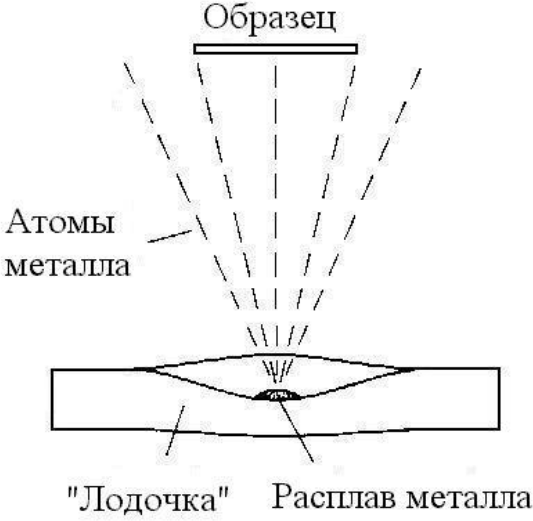
\includegraphics[scale = 0.4]{pictures/boat.png}
\caption{Схема установки для ионно-вакуумного напыления. Воздух откачивается из вакуумной камеры и замещается аргоном при низком давлении; на электрод из соответствующего металла, расположенный вверху камеры, подается высокое напряжение, вызывая газовый разряд; образцы покрываются слоем атомов металла, вырываемых из мишени при бомбардировке ее ионами аргона}
\end{figure}

%\clearpage
\section*{Результаты эксперимента}

Изучаемый образец -- зола рисовой шелухи, содержащая значительное количество силикатов и кремнезема. 

Первый набор снимков был сделан до нанесения металлического слоя на изучаемый образец. Т.к. образец непроводящий, то изначально были выставлены такие настройки прибора, которые бы не приводили к быстрому накоплению заряда на поверхности образца (низкая интенсивность электронного пучка -- PC-low; малое и среднее значение ускоряющего напряжения -- 5, 10 kV). Увеличение ускоряющего напряжения приводит к увеличению контрастности получаемого изображения с использованием детектора вторично-отраженных электронов (SEI). На снимаках видны достаточно крупные агломерационные частицы размером до 200 $\mu m$. Удалось получить малоконтрастное изображение с использованием детектора обратно отраженных электронов (BEI). \par
Затем образец в течении двух минут покрывался золотым напылением в газоразрядной камере. Видимо из-за неоднородного формирования металлического слоя на снимке 000363 видны разные по "засвеченности" зоны образца. При увеличении ускоряющего напряжения до 15 kV изображение получается достаточно "засвеченным" даже после нанесения металлического слоя. Однако снижение интенсивности электронного пучка позволило получить изображение с достаточно высоким масштабных фактором с правильной контрастностью (000362). Также был полученболее качественный снимок с использованием обратно отраженных электронов (000360). Наконец, было сделано изображение при масштабном факторе $900$, на котором хорошо видна игольчатая микроструктура частиц (000365). 

\begin{figure}[!ht]
	\centering
	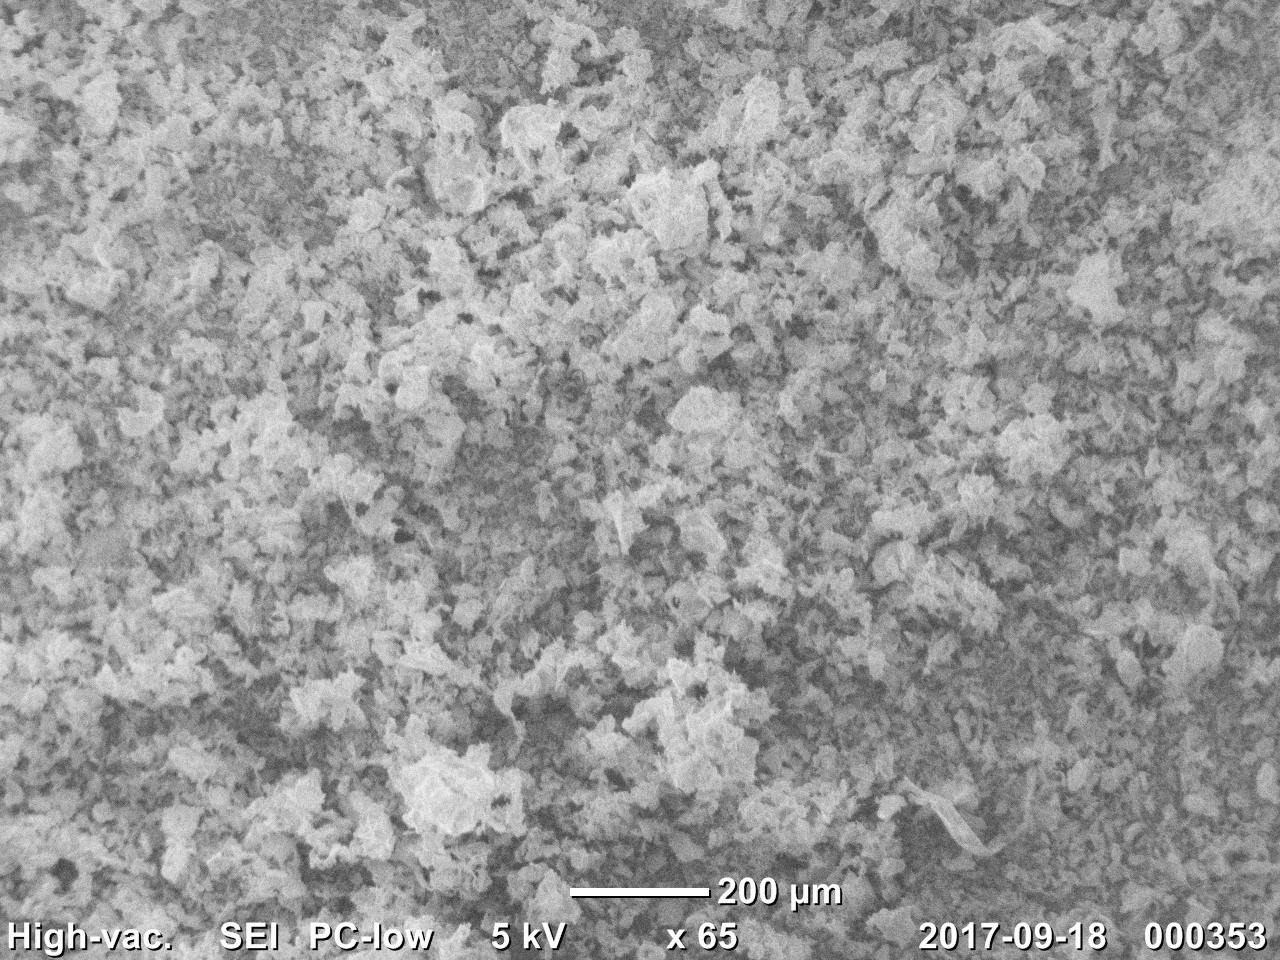
\includegraphics[scale=0.7]{pictures/20170918_000353.jpg}
	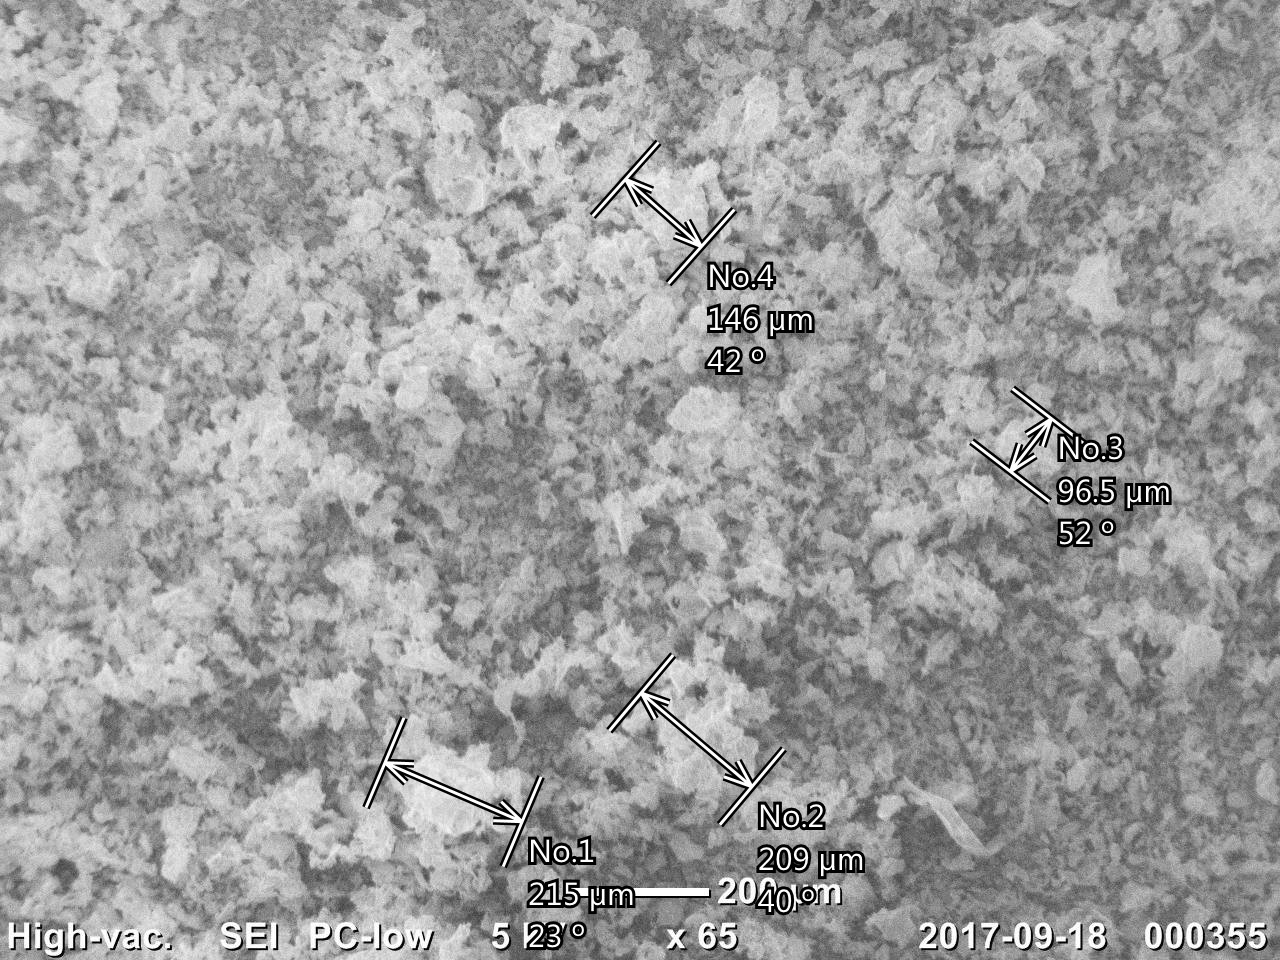
\includegraphics[scale=0.7]{pictures/20170918_000355.jpg}
	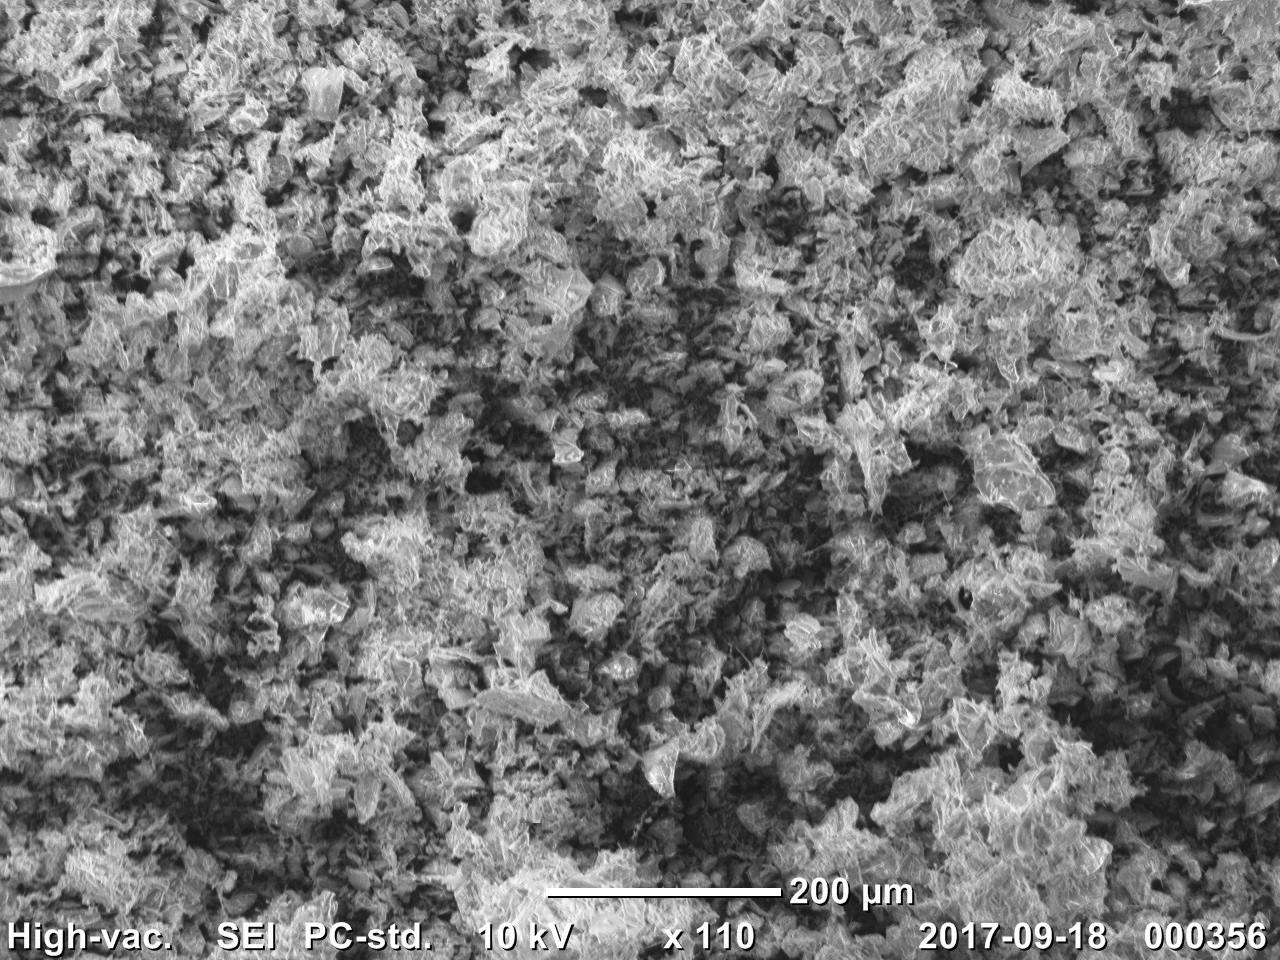
\includegraphics[scale=0.7]{pictures/20170918_000356.jpg}
	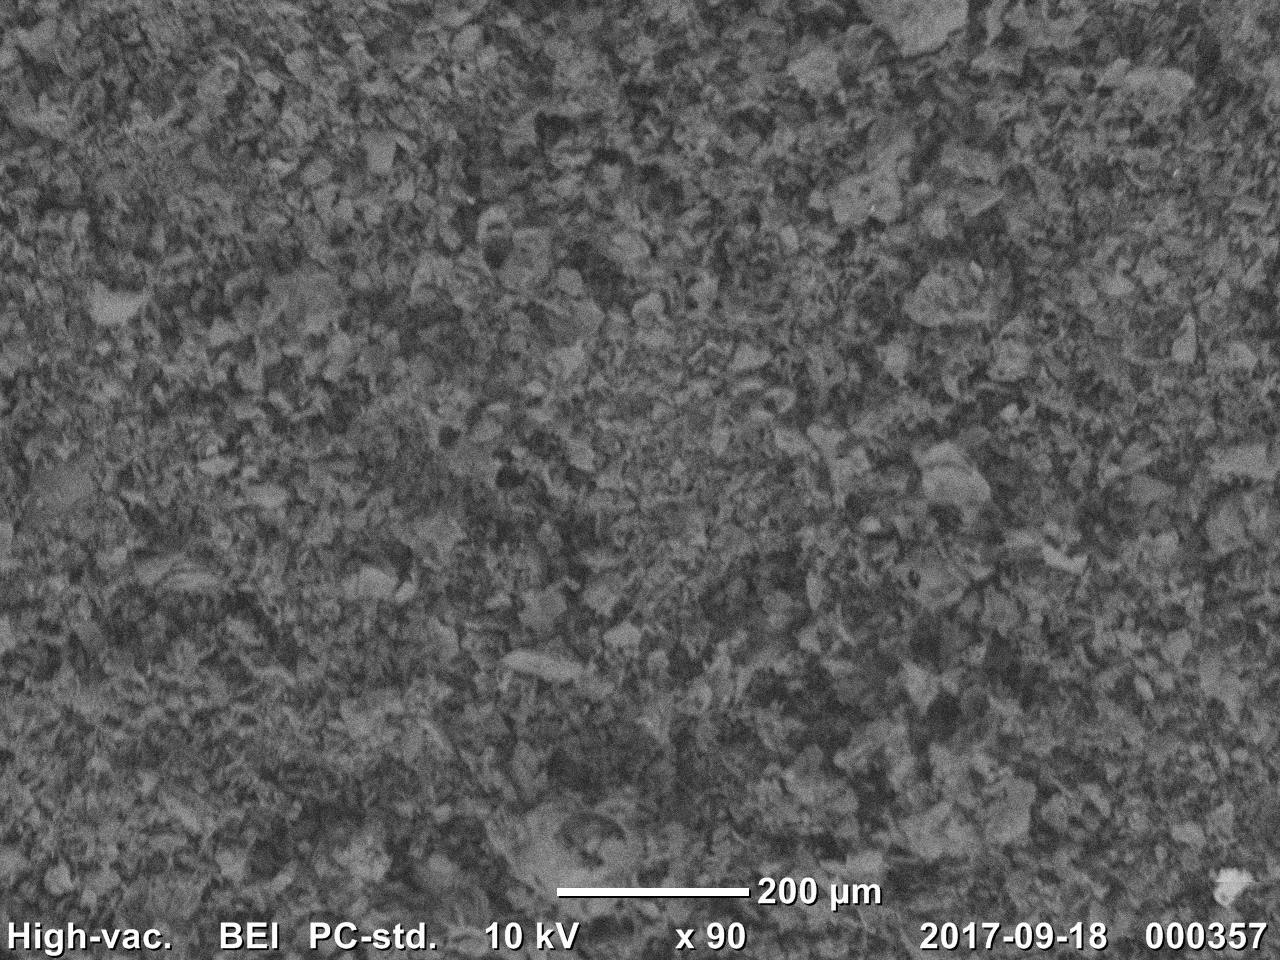
\includegraphics[scale=0.7]{pictures/20170918_000357.jpg}
	\caption{Набор снимков, сделанных до напыления металлического слоя}
\end{figure}

\begin{figure}[!ht]
	\centering
	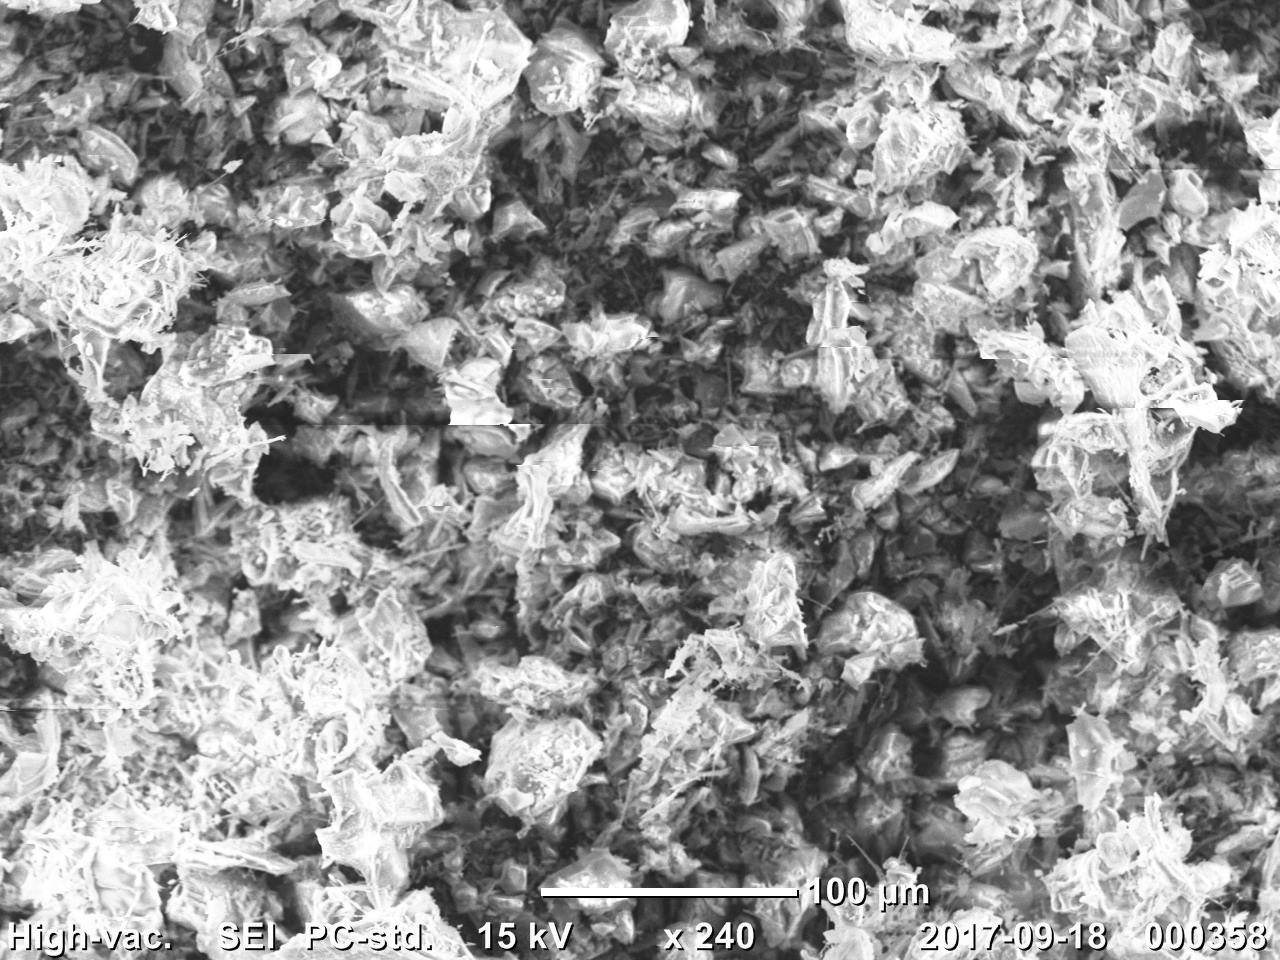
\includegraphics[scale=0.7]{pictures/20170918_000358.jpg}
	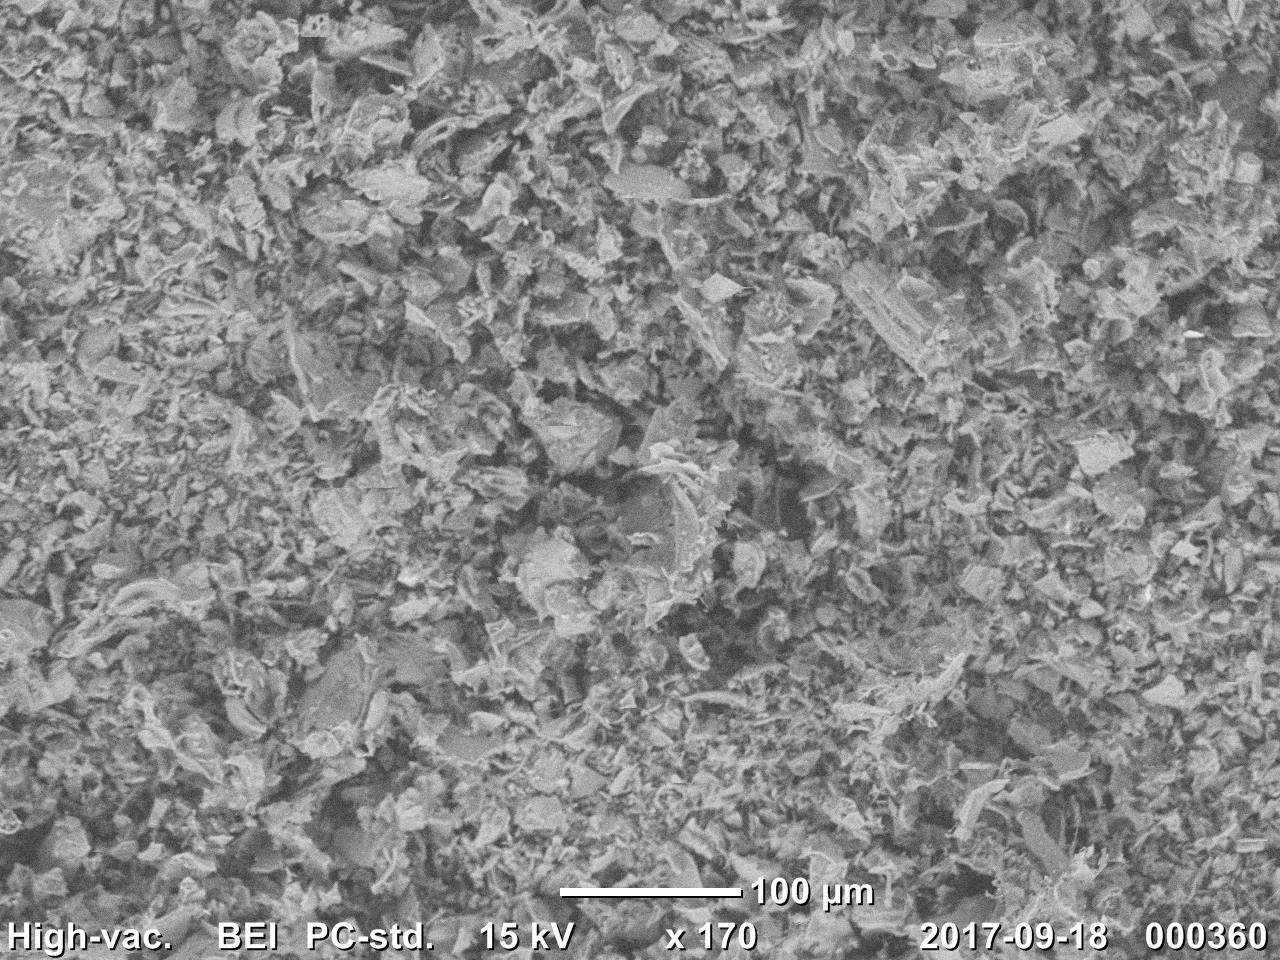
\includegraphics[scale=0.7]{pictures/20170918_000360.jpg}
\end{figure}

\begin{figure}[!ht]
	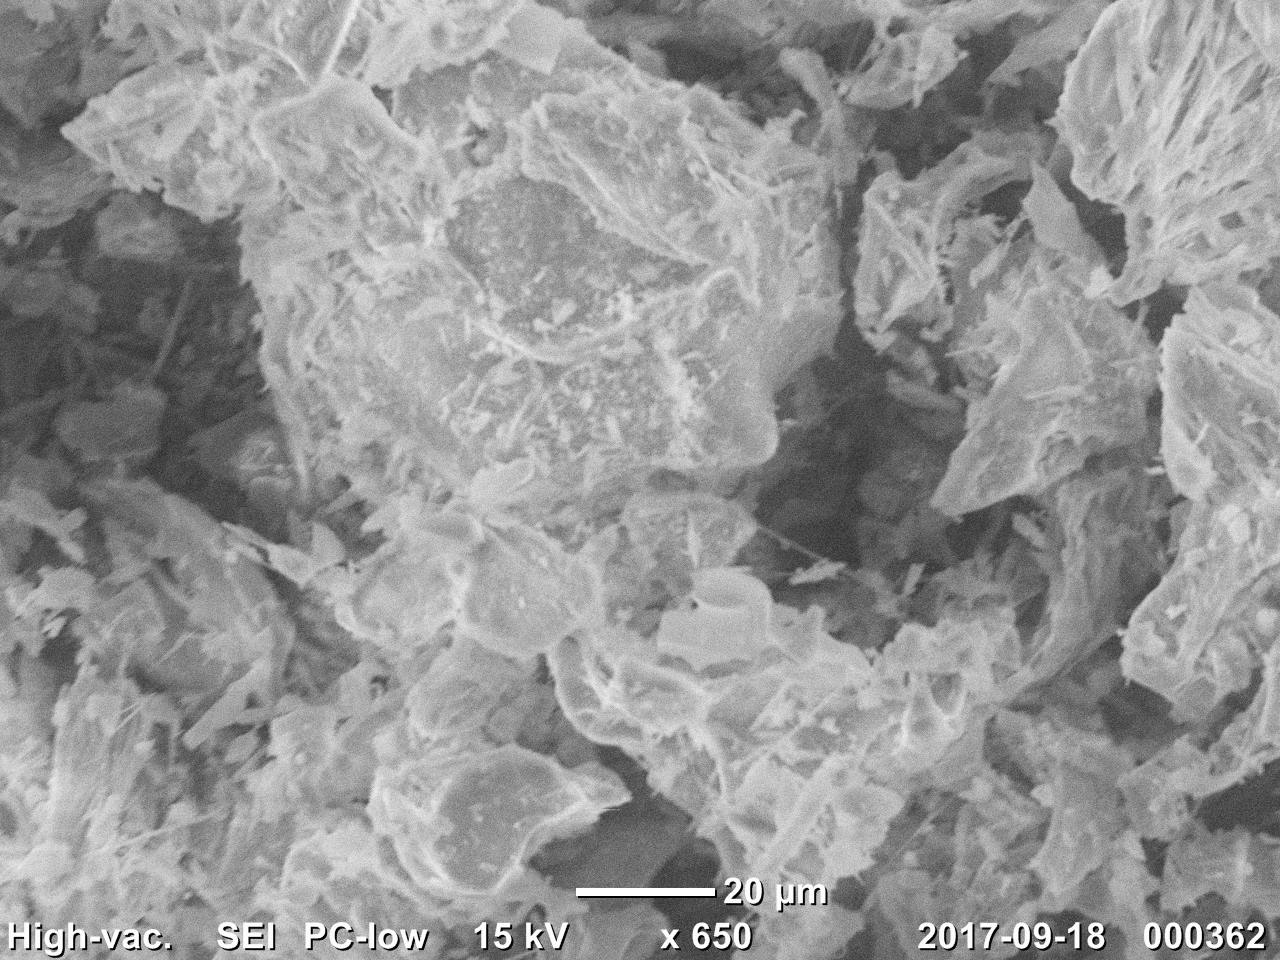
\includegraphics[scale=0.7]{pictures/20170918_000362.jpg}
	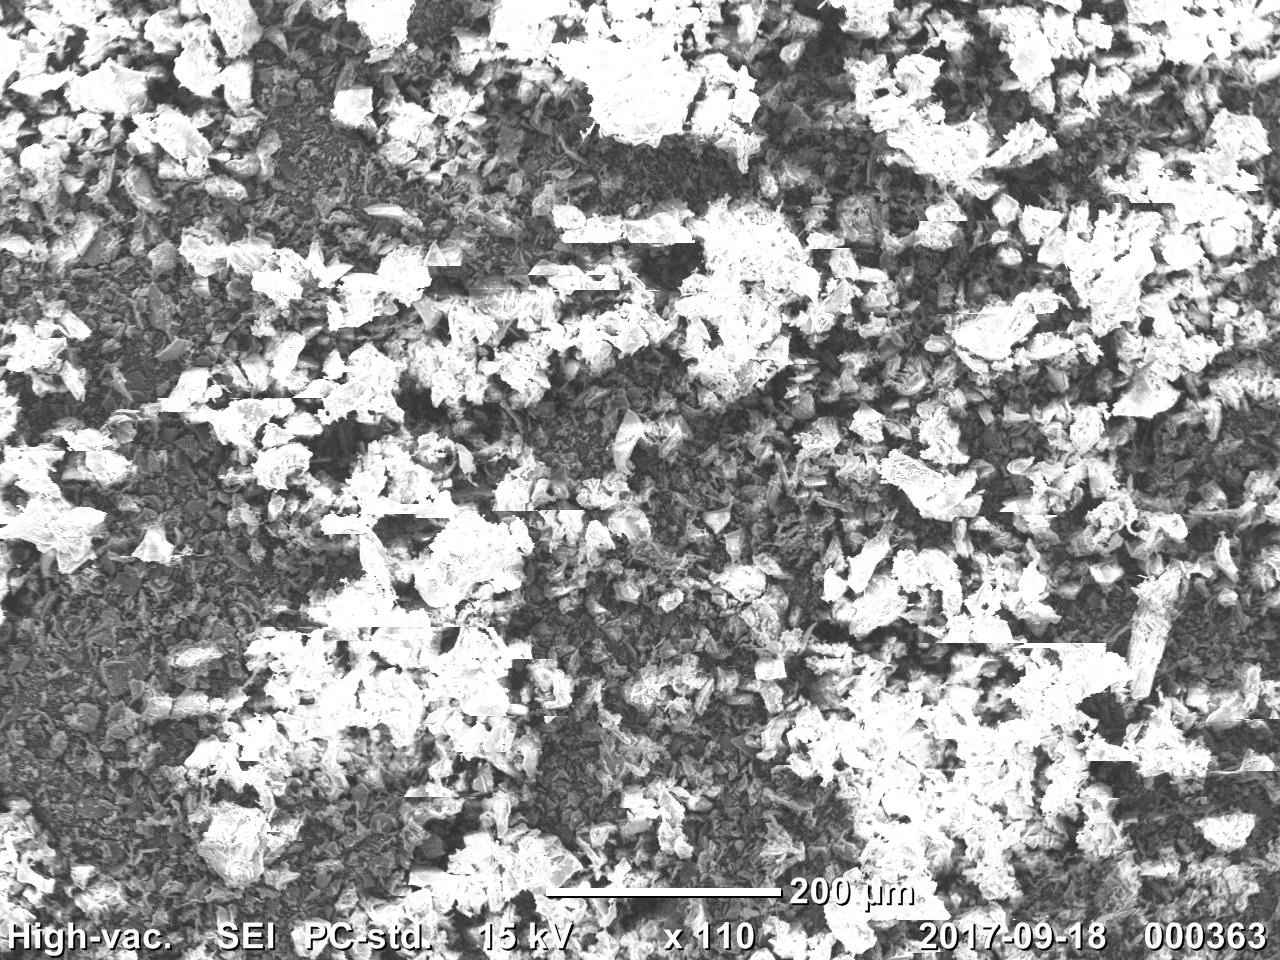
\includegraphics[scale=0.7]{pictures/20170918_000363.jpg}
	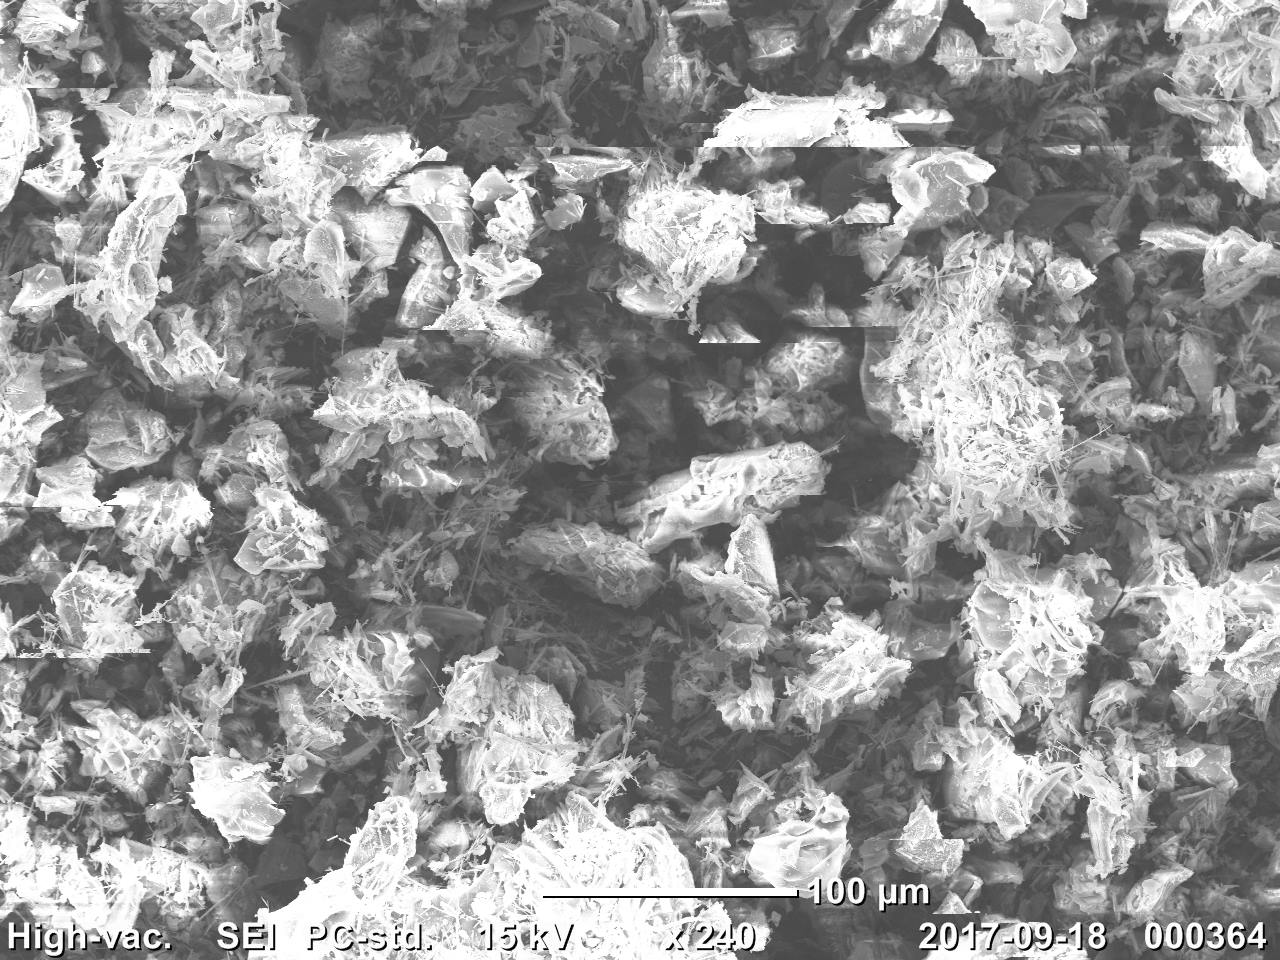
\includegraphics[scale=0.7]{pictures/20170918_000364.jpg}
	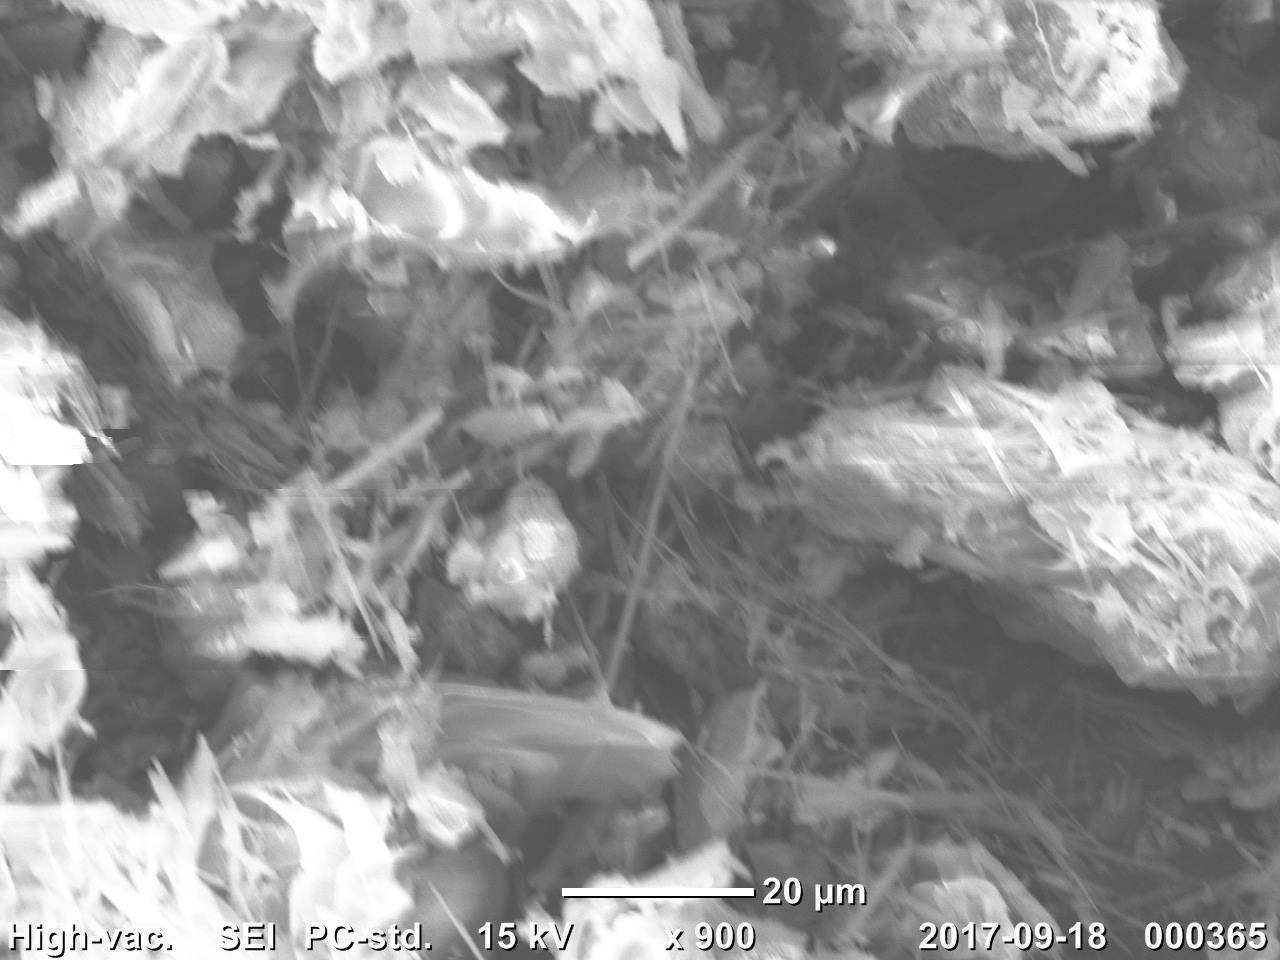
\includegraphics[scale=0.7]{pictures/20170918_000365.jpg}
	\caption{Набор снимков, сделанных после напыления металлического слоя}
\end{figure}

\clearpage
\section*{Список литературы}

\begin{enumerate}
	\item Williams D. B., Carter C. B. (2009). Transmission Electron Microscopy: a Textbook for Materials Science. New York: Springer. 2nd ed.
	\item Reed S. J. B. (1996) Electron microprobe analysis and scanning electron microscopy in geology. Cambridge: University Press.
	\item А. И. Власов, К. А. Елсуков, И. А. Косолапов. (2011). Электронная микроскопия. Издательство МГТУ им. Н. Э. Баумана. 
\end{enumerate}

\end{document}
